\section{Design}
\label{sec:ch3_design}
% New adapter module:

% Consumes prompts created from modified templates (with blend special string to delimit chunks), then extracts and stitches chunks with model's tokenizer, and passes the final forged prompt to LMCache (i.e. CacheBlend's system) for KV cache prefilling with blend enabled.

% This allows flexible chunking granularity simply based on where blend special string is inserted in the frontend prompt template. For example, if chunking is based on context per file/per symbol, the frontend algo can add a blend special string after each of the context snippet fetched during code graph exploration. If on a granularity that is coarser, say per context block (e.g. issue description, repo structure, relevant code), it is also achievable through directly placing the string in frontend prompt after each block.

Our end-to-end system design centers around the concept of \emph{Cached Context}, which provides a simple yet effective approach to maximizing KV cache reuse opportunities in agentic workflows. The key idea is to chunk each prompt at a per-context-object granularity, where a context object corresponds to a code snippet containing a symbol definition, a repository structure tree, or other semantically coherent unit of context.  

\subsection{Cached Context}
\label{sec:ch3_design_cc}
To illustrate the advantage of \textit{Cached Context} over traditional prefix caching, consider the following example. Suppose the agent constructs a prompt after context retrieval, consisting of four parts: system instructions, repository structure, issue description, and relevant code snippet. A naive chunking strategy would treat this prompt as a single unit or divide it into four coarse blocks. With \textit{Cached Context}, we are able to further decompose the context blocks into finer-grainer blocks. The ``relevant code snippets'' block, for example, might contain definitions for multiple symbols retrieved by RepoGraph, where each symbol definition is now its own cache chunk. 

Now consider a subsequent prompt in the same workflow \mytodo{visualize, can just tweak the present slides figure a little}, but with slightly different localization and set of code snippets, while most symbols and other blocks remain the same. Under prefix caching, unless the overlapping content appears from the start of the prompt, the cache cannot be reused. But under \textit{Cached Context}, each overlapping symbol definition is a cache hit regardless of its position. This position-independent reuse is particularly valuable in agentic workflows where the order and combination of context elements frequently varies. 

\subsection{System Architecture}
\label{sec:sysarch}
Figure~\ref{fig:system_arch} illustrates the overall architecture of our end-to-end system. The design prioritizes modularity and extensibility, allowing components to be developed and tested independently. Design details per module are as follows:

\subsubsection{Frontend: RepoGraph + Agentless}

We deploy RepoGraph as the frontend context retrieval algorithm and integrate it with the Agentless procedural framework. Agentless follows a three-step routine:
\begin{enumerate}
    \item \textbf{Localize}: Given an issue description, identify the files and code regions most likely to require modification.
    \item \textbf{Repair}: Generate candidate patches for the localized regions.
    \item \textbf{Rerank}: Evaluate and rank the candidate patches, selecting the most promising one for submission.
\end{enumerate}

RepoGraph enhances the localization phase by providing repository-aware context. Rather than relying solely on file-level search, Agentless can query RepoGraph's code graph to retrieve symbol definitions, call chains, and structural information. This integration ensures that the LLM receives semantically complete context---for example, when localizing a bug in a function, the model also receives definitions of all symbols referenced by that function.

To enable cached context, we modify Agentless's prompt generation routine to explicit context objects, therefore exposing chunk boundaries to the backend adapter without affecting the semantic content of the prompt.


\begin{figure}[ht]
\centering
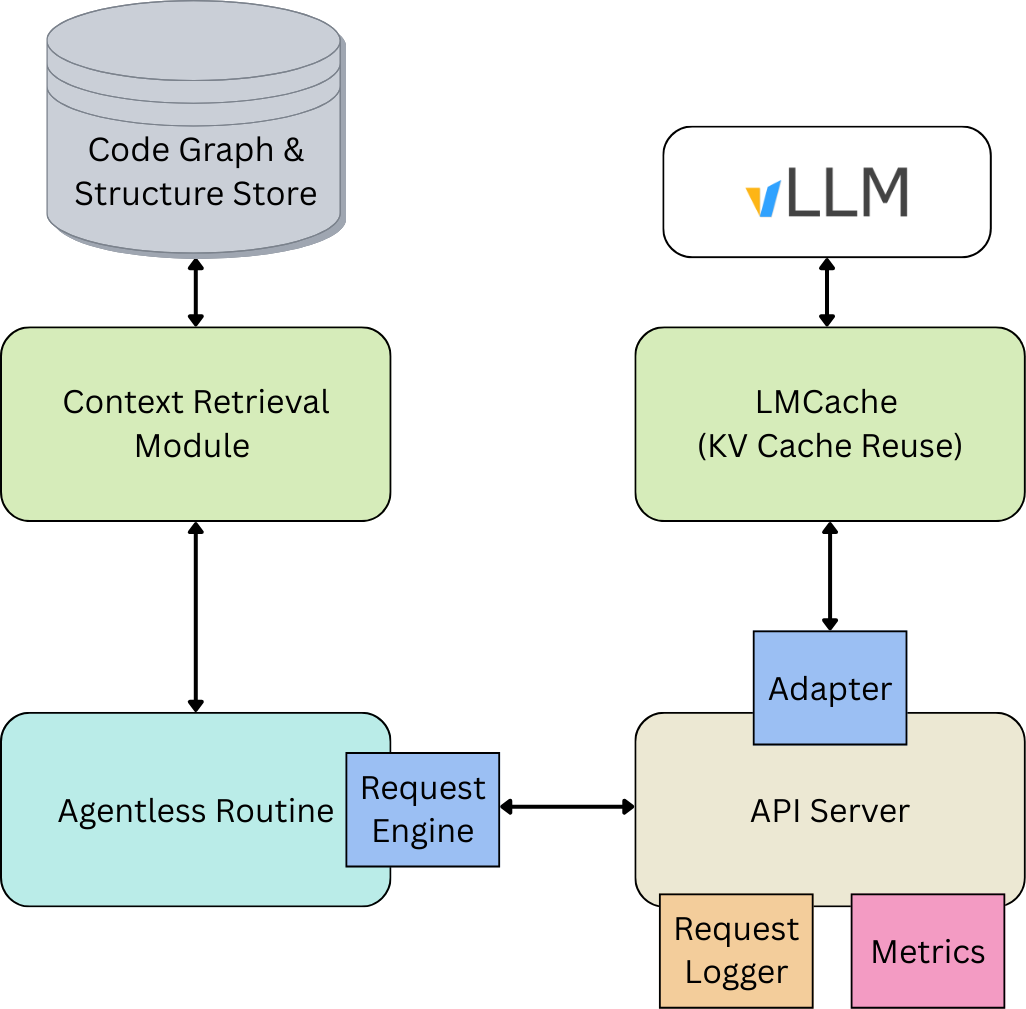
\includegraphics[width=0.75\linewidth]{graphs/E2E sys design.png}
\vspace{0.1in}
  \caption{\small End-to-end system architecture}
 \label{fig:system_arch}
 \vspace{-0.15in}
\end{figure}

\subsubsection{Backend: API Server with CacheBlend}

The backend consists of an API server that serves as the entry point for frontend requests. The server hosts the LLM inference engine (vLLM) with LMCache integration, which implements the CacheBlend algorithm for position-independent KV cache reuse. When a request arrives, the server:
\begin{enumerate}
    \item Parses the chat messages from the request.
    \item Passes the messages through the adapter module (described below) for tokenization and chunk extraction.
    \item Forwards the processed prompt to the LLM engine with CacheBlend enabled.
    \item Returns the generated response to the client.
\end{enumerate}

This modular design ensures that any compatible frontend can benefit from cached context without modification beyond expliciting context objects.


\subsubsection{Adapter Module}

The adapter module serves as the bridge between the frontend prompt format and the backend cache system. Its responsibilities include:
\begin{enumerate}
    \item \textbf{Chunk extraction}: Identifying and retrieving individual context objects.
    \item \textbf{Tokenization}: Encoding each chunk using the model's tokenizer, as well as the correct handling of models with custom tokenization schemes (e.g. Devstral).
    \item \textbf{Chunk stitching}: Reassembling the tokenized chunks to produce the final prompt token sequence.
\end{enumerate}

The adapter's design allows for flexible chunking granularity based on frontend prompt template and user preference. For example, if chunking is based on context per symbol, the frontend adds a delimiter after each code snippet fetched during code graph exploration. If coarser granularity is desired (e.g., per context block), delimiters can be placed only between major sections of the prompt. This provides robustness against various workload patterns and different optimal chunk sizes. 

\subsection{Local Store for Precomputed Data}
\label{sec:local_store}

Computing the code graph and repository structure from scratch for every task instance incurs significant latency overhead. RepoGraph's graph construction involves parsing all source files using tree-sitter, identifying symbol definitions and references, and building the dependency graph. For large repositories, this process can take several minutes.

To address this, we introduce a local store that caches these large data structures. The store is keyed by repository ID and commit hash, ensuring that cached data remain valid across tasks targeting the same codebase state. This optimization is particularly valuable when processing multiple issues against the same repository (common in benchmark evaluations like SWE-bench) or when the same repository is revisited across different agent sessions.

\subsection{Request Logging and Replay}
\label{sec:request_logging}

To support debugging, profiling, and reproducible experimentation, the API server includes a request logging module. During a server session, all incoming requests and their corresponding responses are captured and stored as a local trace file. 

This transparency enables inspection of which stage during the Agentless routine may have caused a performance bottleneck. For example, if localization prompts consistently exhibit low cache hit rates, the prompt template can be adjusted to improve context alignment across requests.

In addition, the server supports a \textbf{replay} functionality that parses requests from any trace file and simulates the workload internally. This feature enables:
\begin{itemize}
    \item Evaluation on captured traces from real agentic workloads without re-running the full agent pipeline.
    \item Modularized testing through synthetic small traces that exercise specific caching scenarios.
    \item A/B comparison of different caching configurations on identical workloads.
\end{itemize}

Both capabilities are desirable for developing a production-ready system, as they allow performance analysis and optimization to proceed independently of the agent's decision-making logic.

\section{Implementation}
% \frank{mention tweaks on repograph and context retrieval for copilot arena here}
Beyond the core architecture, several implementation optimizations improve the system's robustness and performance.

\subsection{Context Truncation}
\label{sec:context_truncation}

For complex coding tasks involving multiple files and nested dependencies, it is possible for the frontend to exceed the model's token limit when constructing a prompt. Originally, prompts were naively truncated at the end when the token limit was reached. This approach frequently results in important instructions (such as output format requirements or validation criteria) being omitted from the prompt. Even when the LLM receives sufficient context to understand the problem, it may underperform due to missing instructions.

\mytodo{adapt visualization from pres slides}

Out solution leverages the model’s tokenizer to calculate the tokens length of each context block and the prompt template. Then before constructing the prompt, the last context block is truncated to exactly fit the remaining token budget, so that the critical pieces on the template will stay intact and instructions will be passed to the LLM as desired. This improves the reliability of the generated patches when the context is long.
